\chapter[Evaluation]{Evaluation}
\label{cp:evaluation}

{
	\parindent0pt
	This chapter presents the scenarios and criteria employed in the evaluation of our implementation. \autoref{sec:benchmark_scenarios} introduces a series of benchmarking scenarios, which have been chosen to reflect distinct simulation characteristics appearing in real-world applications.

	Subsequently, \autoref{sec:metrics} defines the evaluation metrics applied to these benchmarks. The metrics are intended to provide comparability between simulation runs with dynamic tuning intervals and to the baseline runs with static tuning intervals.

	Together, the benchmarking scenarios and evaluation metrics provide a framework for assessing the performance and reliability of the proposed strategies.
}


\section{Benchmarking Scenarios}
\label{sec:benchmark_scenarios}
As to not limit our analysis to one specific simulation setting, we use a selection of benchmarking scenarios. These represent different structures as they may be used in real-world applications.
The heating-sphere and exploding-liquid scenarios are identical to the ones given by Newcome et al., the configuration files have been adapted and parametrized for use in this thesis \cite{Newcome2025}.
The other scenarios are are taken from the AutoPas \texttt{md-flexible} example. %TODO: citation


\pgfplotsset{
	colormap={fast}{
			rgb255(0cm)=(14,14,119);
			rgb255(0.17159223942480895cm)=(61,117,206);
			rgb255(0.2984914818394138cm)=(90,189,243);
			rgb255(0.4321287371255907cm)=(175,237,234);
			rgb255(0.5cm)=(229,240,196);
			rgb255(0.5882260353170073cm)=(244,212,129);
			rgb255(0.7061412605695164cm)=(236,158,80);
			rgb255(0.8476395308725272cm)=(204,89,40);
			rgb255(1cm)=(150,19,30);
		}
}

\newcommand{\fastcolorbar}{%
	\centering
	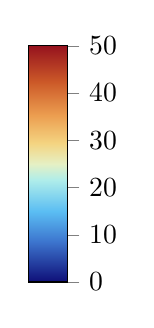
\begin{tikzpicture}
		\pgfplotscolorbardrawstandalone[
			colorbar,
			colormap name=fast,
			point meta min=0,
			point meta max=50,
			colorbar style={
					height=3cm,
					ytick={0,10,...,50},
					tick align=outside,
					tick pos=right,
				},
		]
	\end{tikzpicture}

	\begin{tikzpicture}
		\node[anchor=north, align=center] at (0,0) {\si{F^{*}}};
	\end{tikzpicture}
}

\newcommand{\fastcolorbarhor}{%
	\centering
	\begin{tikzpicture}
		\node[anchor=east, align=center] at (-0.25cm,-0.25cm) {\si{F^{*}}};
		\pgfplotscolorbardrawstandalone[
			colorbar horizontal,
			colormap name=fast,
			point meta min=0,
			point meta max=50,
			colorbar style={
					width=3cm,
					xtick={0,10,...,50},
					tick align=outside,
					tick pos=top,
					xticklabel pos=top,
				},
		]
	\end{tikzpicture}
}


\subsection{Equilibrium}
\label{subsec:equil}
In the equilibrium scenario, particles with initial velocity $0$ are packed tightly into a cube with periodic boundary conditions. The particles interact with each other and the grid structure loosens up, but ultimately an equilibrium is reached in which no rapid changes in velocity occur anymore. After some initial relaxation of the grid structure, there is no further scenario change expected. Therefore, no additional tuning phases should be needed, as the optimal configuration is not expected to change.


\begin{figure}[htpb]
	\centering
	\begin{subfigure}[c]{.3\textwidth}
		\includegraphics[width=\textwidth]{equilibrium/render/t0.png}
		\subcaption{Iteration \num{0}} % 0, 0
	\end{subfigure}%
	\begin{subfigure}[c]{.3\textwidth}
		\includegraphics[width=\textwidth]{equilibrium/render/t10000.png}
		\subcaption{Iteration \num{10000}} % 10000, 10
	\end{subfigure}%
	\begin{subfigure}[c]{.3\textwidth}
		\includegraphics[width=\textwidth]{equilibrium/render/t50000.png}
		\subcaption{Iteration \num{50000}} % 50000, 50
	\end{subfigure}%
	\hfill\begin{subfigure}[c]{.08\textwidth}
		\fastcolorbar
	\end{subfigure}
	\label{fig:evolution_equil}
	\caption{Evolution of the simulation state in the equilibrium scenario.}
\end{figure}


\subsection{Exploding Liquid}
Similarly to the equilibrium scenario, the exploding liquid scenario starts of with the particles packed into a cuboid with periodic boundaries. The cuboid explodes in $y$-direction, collides with the boundary and finally settles into an equilibrium state spread out over the whole simulation space. If a single AutoTuner instance is used for the whole domain, the rapid changes in particle positions and heterogeneous particle distribution make finding an optimal configuration very hard. However, if the domain is split up into multiple independent AutoPas instances on different MPI nodes, each AutoTuning instance can independently find an optimal configuration for its part of the domain. By this, the simulation domain can be split up into regions that have been affected by the \enquote{explosion} and regions that no particles have entered yet.

\label{subsec:expl}
\begin{figure}[htpb]
	\centering
	\begin{subfigure}[c]{.25\textwidth}
		\newsavebox{\colorbarbox}
		\savebox{\colorbarbox}{
			\fastcolorbarhor
		}
		\usebox{\colorbarbox}%
		\vspace*{-\ht\colorbarbox} %
		\includegraphics[width=\textwidth]{exploding-liquid/render/t0.png}
		\subcaption{Iteration \num{0}} % 0 
	\end{subfigure}%
	\begin{subfigure}[c]{.25\textwidth}
		\includegraphics[width=\textwidth]{exploding-liquid/render/t3000.png}
		\subcaption{Iteration \num{3000}} % 3000, 5.5
	\end{subfigure}%
	\begin{subfigure}[c]{.25\textwidth}
		\centering
		\includegraphics[width=\textwidth]{exploding-liquid/render/t11000.png}
		\subcaption{Iteration \num{11000}} % 11000, 20
	\end{subfigure}%
	\begin{subfigure}[c]{.25\textwidth}
		\centering
		\includegraphics[width=\textwidth]{exploding-liquid/render/t31000.png}
		\subcaption{Iteration \num{31000}} % 31000, ?? 
	\end{subfigure}
	\label{fig:evolution_expl}
	\caption{Evolution of the simulation state in the exploding liquid scenario.}
\end{figure}

\subsection{Heating Sphere}
\label{subsec:hs}
The heating sphere scenario consists of a dense, small sphere of particles. Reflective boundary conditions apply as in the previous scenarios. In the course of the simulation, the temperature rises from $0.1$ to $100$ with a $\Delta \si{T^{*}}=0.1$ every 100 iterations. Additionaly, brownian motion, i.e. random fluctuations in particle positions are applied \cite{Moerters2010}. The sphere expands with the inrcease in temperature and particles are radiating out from the sphere center.

\begin{figure}[htpb]
	\centering
	\fastcolorbarhor
	
	\begin{subfigure}[c]{.25\textwidth} 
		\includegraphics[width=\textwidth]{heating-sphere/render/t0.png}
		\subcaption{Iteration \num{0}} % 0
	\end{subfigure}%
	\begin{subfigure}[c]{.25\textwidth}
		\includegraphics[width=\textwidth]{heating-sphere/render/t4000.png}
		\subcaption{Iteration \num{4000}} % 4000, 0.4
	\end{subfigure}%
%		\begin{subfigure}[c]{.25\textwidth}
%			\centering
%			\includegraphics[width=\textwidth]{heating-sphere/render/t12000.png}
%			\subcaption{Iteration \num{12000}} % 12000, 1.2
%		\end{subfigure}%
	%	\hspace*{.15\textwidth} 
	\begin{subfigure}[c]{.25\textwidth}
		\includegraphics[width=\textwidth]{heating-sphere/render/t23000.png}
		\subcaption{Iteration \num{23000}} % 23000, 2.3
	\end{subfigure}%
	\begin{subfigure}[c]{.25\textwidth}
		\vspace*{0.1\textwidth}
		\centering
		\includegraphics[width=0.8\textwidth]{heating-sphere/render/t60000.png}
		\vspace*{0.1\textwidth}
		\subcaption{Iteration \num{60000}} % 60000, 6
	\end{subfigure}%
	\label{fig:evolution_hs}
	\caption{Evolution of the simulation state in the heating sphere scenario.}
\end{figure}

\subsection{Falling Drop}
\label{subsec:fd}
\subsection{Spinodial Decomposition}
\label{subsec:sd}

\section{Evaluation Metrics}
\label{sec:metrics}
To compare results between dynamic and static tuning intervals, different metrics can be used.
Firstly, the primary goal is to reduce the total simulation runtime for a range of typical scenarios. As tuning phases spend time in quite suboptimal configurations, a reduction in total runtime is the expected result if our approach reduces the number of tuning phases without spending too many iterations using a suboptimal configuration outside tuning phases.

The metric of total runtime is not particularly fine-grained however, as it only takes into account entire simulation runs. To achieve a more detailed benchmark, we also consider the number of iterations that were running on an optimal configuration. As an approximation to the optimal configuration per iteration we use simulation run with static tuning, a high number of tuning samples and a short tuning interval. Based on this static data we can then rank the configuration our dynamic run chose in terms of \enquote{optimality}.

%Finally, the percentage of tuning iterations might be of interest. Depending on the tuning strategy used, the retuning process can terminate early. % TODO?
%Therefore, the actual number of iterations spent in a tuning phase might be different depending on the iteration in which that phase was started. In such cases, it might be beneficial to have more 

